\documentclass{weeklyreport}
\usepackage[utf8]{inputenc}

%%% Template Usage
% 1. Go to "All Projects" and make a copy in Overleaf,
% or download the source to modify locally.
% 2. Fill in your name
% 3. Set the reportdate to Monday of the current week


\title{Progress Report}
\author{Edris Qarghah}

\DTMsavedate{reportdate}{2020-07-13}
\date{Week of \DTMusedate{reportdate}}

\begin{document}

\maketitle

\newpage

\section*{Weekly Goals}


\begin{itemize}
    \item Toy Network
    \begin{itemize}
        \item Create a more robust network generation process (e.g., ensuring MST).
        \item Simulate network activity.
        \item Measure activity from specific nodes and generate a resulting time series.
        \item Develop tools for tomography and anomaly detection.
        \item Improve visualization of networks.
    \end{itemize}
    \item Explore real network to understand how to better model it.
    \begin{itemize}
    	\item Hub and spoke approach to network generation?
    \end{itemize}
\end{itemize}

\section*{Daily Log}

\subsection*{\weekday{0}}

\begin{itemize}
    \item Network Analytics Discussion meeting.
    \begin{itemize}
    	\item Met Shawn, Petya, Soundar and Tommy and learned a bit about what each is working on (apparently Painless is NOT painless).
    	\item Shared my progress from last week.
    	\item Added my weekly progress report presentation to SAND drive (meeting notes and personal folders) and will do so in the future.
    	\item Discussed the possibility of having multiple classes of nodes with differing levels of connectedness (e.g., hubs that have many connections and destinations that have only a few).
    \end{itemize}
    \item Explored \href{https://perfsonar.uc.ssl-hep.org/}{PerfSonar visualization} for a better sense of what a network actually looks like.
\end{itemize}

{\centering 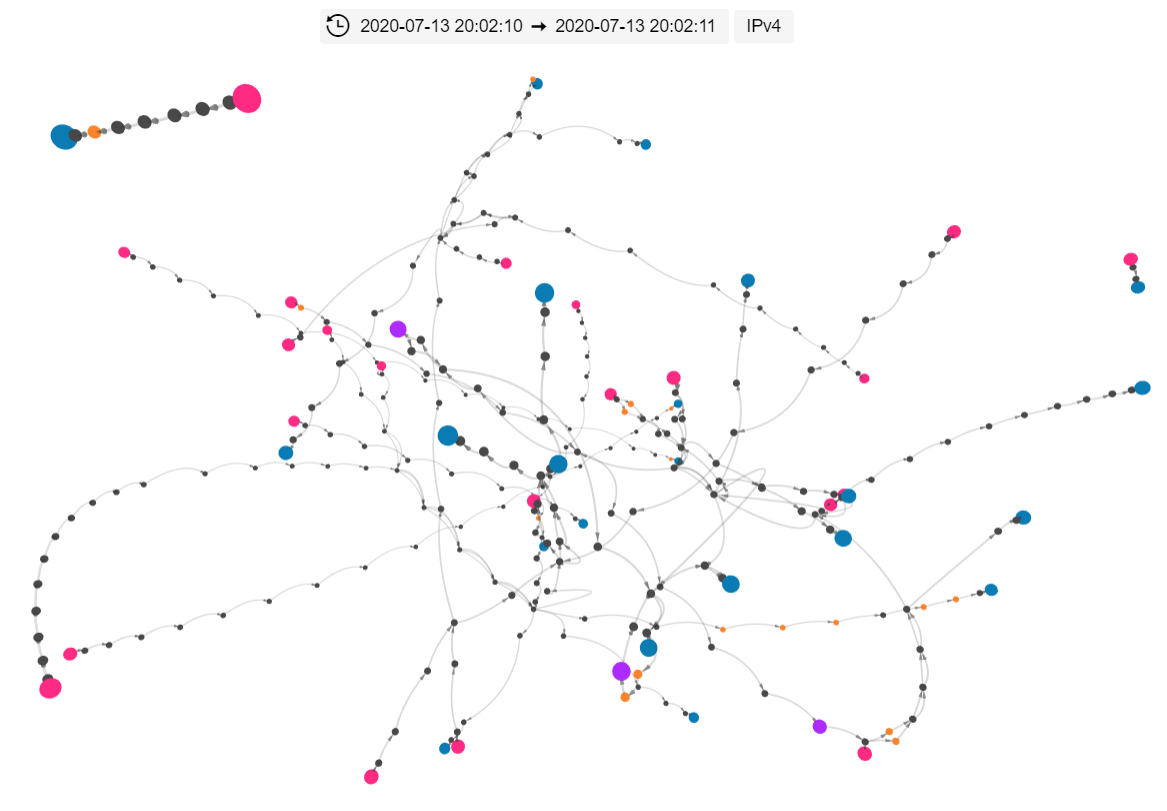
\includegraphics[width=\linewidth]{week_2/Annotation 2020-07-13 163617.png}}

\begin{itemize}
    \item Ilija provided a helpful overview of how packet tracing works and I \href{http://users.cs.cf.ac.uk/Dave.Marshall/Internet/node77.html}{read up on it to supplement/solidify my understanding}:
	\begin{itemize}
		\item TCP packets have a Time To Live (TTL) which determines how many hops they can make before being discarded. This prevents packets from travelling the internet forever, as each hop decrements the TTL counter by 1.
		\item When a TTL counter reaches zero, it is dropped and a message is sent back to the source to indicate where that happened.
		\item Trace Routes leverage this by sending repeated packets to the same destination with incrementally higher TTL (i.e., the first one dies after the first hop, the second after the second hop, etc.). As each time TTL expires an ICMP "time exceeded" message is sent back with the info of where it happened, we can map out nodes that are one, two, three, etc. hops away, until we arrive at the destination.
		\item Notes:
		\begin{itemize}
			\item These are separate packets, so we are not guaranteed that the third hop that the TTL=3 packet died at is the same as the third hop made by the TTL=4 packet. As such, the path drawn by a trace route may depict hops between nodes that are not actually connected to one another!
			\item It's possible that a node is visited twice on a trace-route, which is called a self-loop. This could happen, for example the TTL=6 packet took a different route and died at the same node as TTL=3, or it could be that there was a routing error that really meant that it passed through the node at TTL=3 but the fifth node decided that node was the best route and sent it back there again.
			\item Some nodes (i.e., those behind firewalls at CERN and the like) will not send return messages when dropping a packet, but may still forward a packet that still has TTL. The dropped packets that didn't receive a response are orange in the PerfSonar visualization.
		\end{itemize}
	\end{itemize}
	\item Discussed with Ilija the shape of the network (i.e., some bottleneck links like the transatlantic one, some highly connected regions, like Europe).
    \item Reviewed Suchant's \href{https://docs.google.com/presentation/d/1XBkRZPMpXt2LNcMdrFH1u8UH91dsFsn_SKXPIySYsxw/edit#slide=id.p}{work and diagrams} again. He was using ElasticSearch to explore the paths that were being taken on the network and understand them, so that he could identify paths that were performing poorly and flag them.
\end{itemize}


\subsection*{\weekday{1}}

\begin{itemize}
    \item Finalized and pushed refactoring from previous day.
    \item Spoke with Ilija about packet loss and \href{https://en.wikipedia.org/wiki/Packet_loss}{read about it further} to solidify my understanding:
    \begin{itemize}
    	\item Packet loss is a measure of link quality that can be diminished for a wide variety of reasons (e.g., induction errors, temperature swing, dirty fiber).
    	\item When a packet is lost, the bandwidth of that route is temporarily reduced by 50\%. With stable performance, it is increased back again in 5\% increments, which can take a long time to get back up to full capacity.
    	\item A link with 1\% packet loss is effectively dead, unless the latency is VERY small. Data is buffered on both sides of the communication and a lost packet means that the packet needs to be resent, messing with the buffering (which is FILO).
    	\item \textit{Big Takeaway:} The detrimental impact of packet loss is proportional to the latency of the connection.
    \end{itemize}
    \item Created SSH key and \href{https://www.ci-connect.net/profile}{profile for CI-connect} and requested access to \href{https://www.ci-connect.net/groups/root.slate-training}{slate training}.
    \item Uploaded passport photo to Workday.
    \item Had an unproductive diversion trying to update the Jupyter lab python kernel on the ML platform. Deemed the pay-off of having 3.6+ not worth sinking additional time into it.
    \item Learned about \href{https://www.youtube.com/watch?v=5wCZqdCDafc}{k-connected graphs} and ensured that my graphs are at least 1-connected.
    \item Developed a means of creating "hub" nodes recursively to serve as a backbone for the network.
\end{itemize}

\subsection*{\weekday{2}}

\begin{itemize}
    \item Accidentally lost all work from previous day because I overwrote ML instance. Created a new one, rewrote and enhanced code, including:
    \begin{itemize}
    	\item Ensuring k-connectivity.
    	\item Creating hub nodes recursively.
    	\item Allowing parameters to be set for network generation.
    	\item Generating names and saving all graphs that are generated.
    \end{itemize}
    \item Installed Pandoc to try to enable using Jupyter lab as documentation but was not able to get latex to render.
    \item Attended SLATE tutorial.
%    \begin{itemize}
%    	\item Confirm login
%    	\item Lincoln demo
%    	\begin{itemize}
%    		\item Federated Operations (Compute, Data and proposed Service endpoint)
%	    	\item 'slate app list' (curated application catalog)
%    		\item Demo of glubus-connect-v4 ('slate app get-conf global-connect-v4' | vim -)
%    		\item 'head -n1 lincoln-globus-creds'
%    		\item CI login based identification
%    		\item 'slate secret create' (kubernetes concept)
%    		\item 'slate instance info instance_Dw... | less'
%    		\item app.globus.org > Endpoints > slateci#sl-um
%    	\end{itemize}
%		\item Chris talk
%    	\begin{itemize}
%	    	\item federated > give responsibliity to experts at other sites
%    		\item clusters by default only give access to creating organization
%    		\item other orgs can be granted access to run their own apps
%    		\item Slate places application within separate namespaces.
%    		\item Helm gives templating engine and other conveniences	
%    	\end{itemize}
%    	\item Chris live demo (slateci.io)
%    	\begin{itemize}
%    		\item Web Portal (link at top)
%    		\item Can view but needs login for more	
%    	\end{itemize}
%		\item kubernetes documentation
%    	\begin{itemize}
%    		\item concepts
%    		\item tasks
%    		\item tutorials	
%    	\end{itemize}
%    \end{itemize}
\end{itemize}

\subsection*{\weekday{3}}

\begin{itemize}
    \item Discussed packetloss distribution with Ilija:
    \begin{itemize}
    	\item Packets are sent 10 times a second, for a total of 600 over a minute to determine packetloss rates.
    	\item Ilija showed me to access useful data visualizations in Kibana (pictured below, log of count of packetloss rate (i.e., count of times in 30 days that 2\% of packets were lost).
	\end{itemize}

    {\centering 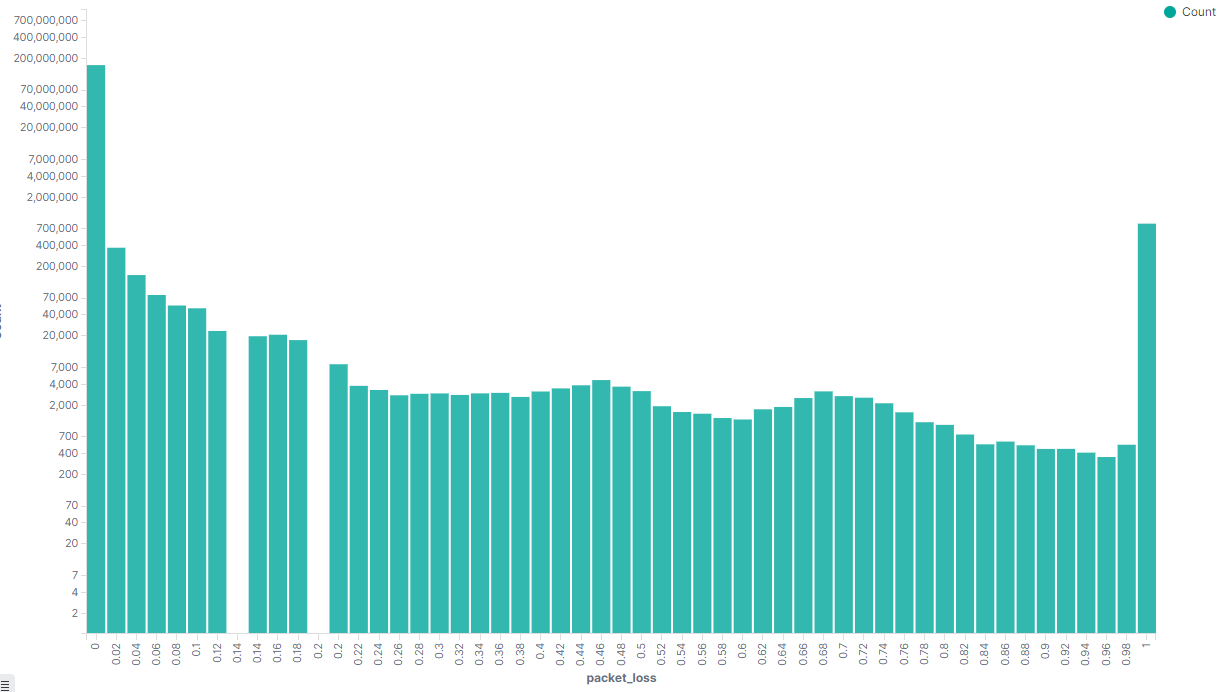
\includegraphics[width=\linewidth]{week_2/packetloss.png}}
    
	\begin{itemize}
    	\item The distribution was heavily skewed toward 0 with a spike at 1, due to dead connections.
	\end{itemize}     
	\item Exported packetloss data, cleaned data and took the square root of the count in each band before using it to create a distribution (the count was too heavily skewed for an effect to be likely/visible on the scale we're working with, but the log flattened things out too much; the square root was a decent middle ground).
	\item Randomly selected packetloss rate for each edge based on the distribution derived from the Kibana data.
	\item Improved network graphs:
	\begin{itemize}
		\item Added network name, so that interesting graphs can be pulled up again (as they are being saved.
		\item Added color coding for PerfSonar, Hub nodes, sources and destinations (the last two haven't been implemented on the network side yet).
	\end{itemize}

    	{\centering 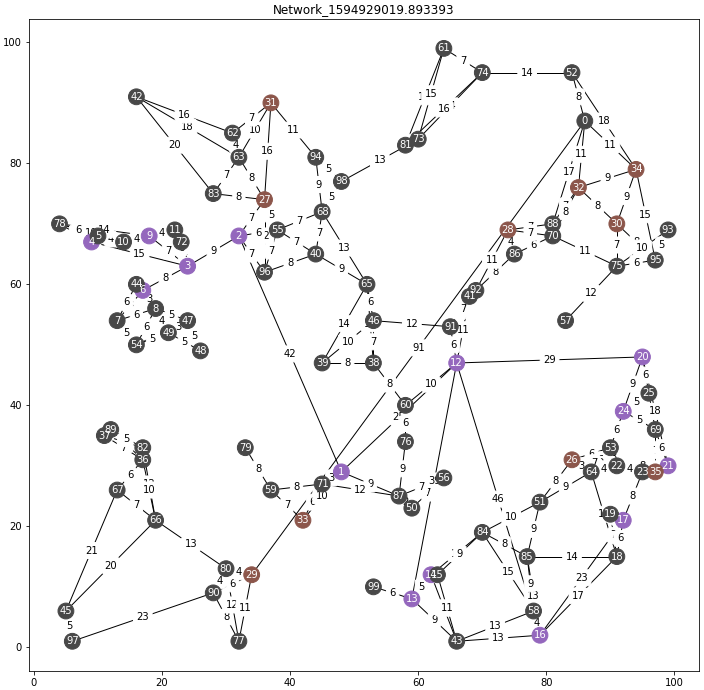
\includegraphics[width=\linewidth]{week_2/NetworkColor.png}}
    
    \begin{itemize}
		\item Tested displaying packetloss rate instead of latency of edges.
	\end{itemize}
\end{itemize}

{\centering 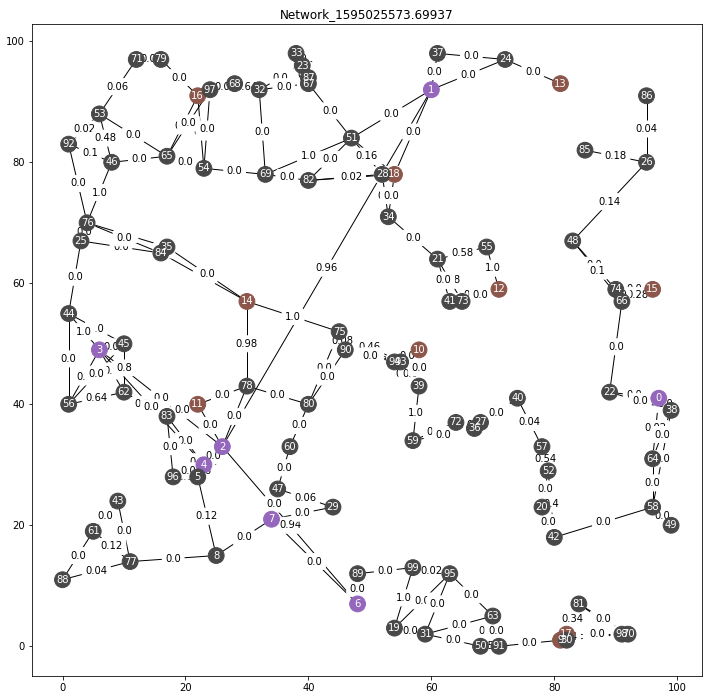
\includegraphics[width=\linewidth]{week_2/NetworkPacketloss.png}}


\subsection*{\weekday{4}}

\begin{itemize}
	\item Fixed bug where first hub node wasn't being connected to it's children.
\end{itemize}

    {\centering 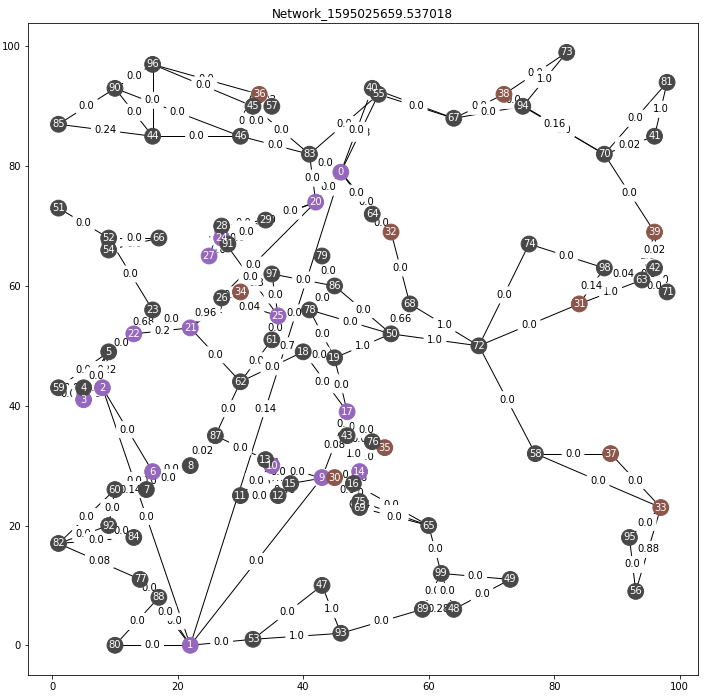
\includegraphics[width=\linewidth]{week_2/NetworkZero.png}}

\begin{itemize}
    \item Created a list of PerfSonar nodes and found the shortest distance between each pair, based on latency.
    \item Created progress report deck and updated this document.
\end{itemize}

\section*{Achievements}
\subsection*{I learned about...}
\begin{itemize}
	\item Slate and its use.
	\item Packet tracing and related complications/considerations.
	\item Packet loss and its causes.
	\item Visualizations in Kibana.
	\item K-connected graphs.
	\item NetworkX's functionality around:
	\begin{itemize}
		\item Node coloring.
		\item Finding shortest path.
		\item K-connected-edge augmentation.
	\end{itemize}
\end{itemize}

\subsection*{I created...}
\begin{itemize}
	\item More robust networks:
	\begin{itemize}
		\item Generation refactored into separate script and parameterized.
		\item Always k-connected (configurable).
		\item Nodes that serve as hubs and branch (forming a network backbone) recursively to a specified depth.
		\item PerfSonar nodes (configurable).
	\end{itemize}
	\item Better visualizations of networks:
	\begin{itemize}
		\item Color coded nodes.
		\item Figures named after graph, to make referencing/exploring graphs easier in the future.
	\end{itemize}
	\item Weekly progress report slides and document (I know this is the same every week, but it is a pretty significant chunk of time and work that I am proud of).
\end{itemize}

\pagebreak
\section*{Roadblocks}

\subsection*{Questions}

\begin{itemize}
	\item The hub system seems to work well for ensuring there are some longer connections. What would be some other good ways to create clustering while maintaining broader connectivity?
	\item Should higher hubs (i.e., hubs connecting other hubs) be disconnected from lesser nodes entirely?
	\item How connected should nodes of various depths be?
	\item How can I ensure that PerfSonar nodes are well distributed and not too centrally located?
	\item How do I combine latency and packetloss edge data to get meaningful tomography?
\end{itemize}

\subsection*{Problems}

\begin{itemize}
	\item I accidentally overwrote my ML instance.
	\item I was unable to get Jupyter notebook updated to 3.6+ on my ML instance.
	\item I was unable to get LaTex to render from Jupyter notebook.
\end{itemize}

\subsection*{Challenges}

\begin{itemize}
    \item Depicting network branching.
    \item Having graph attributes reflected on the figures drawn (e.g., node coloring).
    \item More broadly, using built-in functions (i.e., shortest path algorithms) on non-standard/custom criteria.
\end{itemize}

\section*{Plans for Next Week}

\begin{itemize}
	\item Learn about tomography strategies.
	\item Develop tomography of static network (e.g., with latency/packet loss)
	\item Simulate network activity.
	\item Generate time series based on that activity.
	\item Learn how this connects to anomaly detection.
	\item Explore how the model can be applied to real network data.
\end{itemize}

\end{document}
